\begin{name}
	{\tenchude}
	{\tendethi}
	{\tentruong}
	{\thoigian}
\end{name}
\caulc
\Opensolutionfile{ans}[ans/11-CK1-THPT-Vinh-Xuan-Vinh-Long-Phan-1]
\begin{ex}%[Câu 1]%[1D1N1-3]
	Điểm $N$ biểu diễn cho góc lượng giác có số đo $\dfrac{31\pi}{36}$ rad nằm ở góc phần tư thứ mấy?
	\choice
	{Thứ I}
	{\True Thứ II}
	{Thứ III}
	{Thứ IV}
	\loigiai{
		Đổi $\dfrac{31\pi}{36}\cdot \dfrac{180}{\pi}=155^\circ$.\\
		Biểu diễn lên đường tròn lượng giác
		\begin{center}
			\begin{tikzpicture}[scale=1, line width=1pt]
				\trucLG
				\pointLG{155}{1}{*}{red}			
			\end{tikzpicture}
		\end{center}
		Vậy điểm $N$ biểu diễn cho góc lượng giác trên nằm ở góc phần tư thứ II.
	}
\end{ex}

\begin{ex}%[Câu 2]%[1D1N3-1]
	Trong các công thức sau, công thức nào \textbf{sai}?
	\choice
	{$\cos 2a={\cos ^2}a-{\sin ^2}a$}
	{\True $\sin 2a={\cos ^2}a-{\sin ^2}a$}
	{$\cos 2a = 2{\cos ^2}a-1$}
	{$\sin 2a=2\sin a\cos a$}
	\loigiai{
		Ta có $\sin 2a=2\sin a\cos a$ nên $\sin 2a={\cos ^2}a-{\sin ^2}a$ sai.
		}
\end{ex}

\begin{ex}%[Câu 3]%[1D1N4-5]
	Hàm số $y=\cot x$ có chu kì tuần hoàn là
	\choice
	{\True $\pi$}
	{$2\pi$}
	{$\dfrac{\pi}{2}$}
	{$\dfrac{3\pi}{2}$}
	\loigiai{
		Hàm số $y=\cot x$ có chu kì tuần hoàn là $\pi$.
	}
\end{ex}

\begin{ex}%[1D1N5-3]%[CTST - Lớp 11 - Ôn tập cuối học kì 1 - Đề 4]%[Bùi Anh Trường]
Nghiệm của phương trình $\cos 2x=1$ là
\choice
{$x=k2\pi, k\in \mathbb{Z}$}
{\True $x=k\pi, k\in \mathbb{Z}$}
{$x=\pi+k 2\pi, k\in \mathbb{Z}$}
{$x=\frac{\pi}{2}+k\pi, k\in \mathbb{Z}$}
\loigiai
{Ta có $\cos 2x=1 \Leftrightarrow 2x=k2\pi \Leftrightarrow x=k\pi,k\in \mathbb{Z}$.
}
\end{ex}

\begin{ex}%[Câu 4]%[1D2N1-5]
	Cho dãy số $(u_n)$ có $u_n=n^2+n$. Tính chất nào sau đây của dãy số $(u_n)$ là đúng?	
	\choice
	{\True Không bị chặn}
	{Bị chặn trên}
	{Biến thiên}
	{Bị chặn}
	\loigiai{
		Dãy số này liên tục tăng khi $n$ tăng và không có giới hạn trên, tức là không bị chặn.\\
		Vậy dãy số $(u_n)$ không bị chặn.
	}
\end{ex}

\begin{ex}%[Câu 5]%[1D2N2-3]
	Cho cấp số cộng $(u_n)$ có số hạng đầu $u_1=-2$ và công sai $d=-7$. Khi đó, số hạng tổng quát của cấp số cộng này là
	\choice
	{\True $u_n=5-7n$}
	{$u_n=-2-7n$}
	{$u_n=-7-2n$}
	{$u_n=7-5n$}
	\loigiai{
		Số hạng tổng quát $u_n=u_1+(n-1)d=-2+(n-1)(-7)=-7n+5$.
	}
\end{ex}

\begin{ex}%[Câu 6]%[1D2N3-2]
	Dãy số nào sau đây\textbf{ không phải} là một cấp số nhân?
	\choice
	{$5$; $10$; $20$; $40$}
	{$3$; $6$; $12$; $24$}
	{$2$; $4$; $6$; $8$}
	{\True $2$; $6$; $18$; $52$}
	\loigiai{
		\begin{itemize}
			\item Dãy số $5$; $10$; $20$; $40$ là cấp số nhân với công bội $q=2$.
			\item Dãy số $3$; $6$; $12$; $24$ là cấp số nhân với công bội $q=2$.
			\item Dãy số $2$; $4$; $6$; $8$ là cấp số nhân với công bội $q=2$.
			\item Dãy số $2$; $6$; $18$; $52$ không là cấp số nhân.
		\end{itemize}
	}
\end{ex}

\begin{ex}%[Câu 7]%[1H4N2-1]
	Khẳng định nào sau đây là \textbf{đúng}?
	\choice
	{Trong không gian, hai đường thẳng cùng song song với một đường thẳng thứ ba thì song song với nhau}
	{Trong không gian, hai đường thẳng song song nhau nếu chúng không có điểm chung}
	{Trong không gian, ai đường thẳng cùng song song với một mặt phẳng thì song song với nhau}
	{\True Trong không gian, không có một phẳng nào chứa cả hai đường thẳng $a$ và $b$ thì ta nói $a$ và $b$ chéo nhau}
	\loigiai{
		Trong không gian, không có một phẳng nào chứa cả hai đường thẳng $a$ và $b$ thì ta nói $a$ và $b$ chéo nhau.
	}
\end{ex}

\begin{ex}%[Câu 8]%[1H4H3-2]
	Cho hình chóp tam giác $S . A B C $. Gọi $P$ và $Q$ lần lượt là trung điểm của $SB$ và $SA$. Khẳng định nào sau đây là đúng?
	\begin{center}
		\begin{tikzpicture}[line join=round, line cap=round, thick,scale=.7]
			\path
			(0,0) coordinate (A)
			(2,-2) coordinate (C)
			(5,0) coordinate (B)
			(1,4) coordinate (S);
			\draw (S)--(A)--(C)--(B)--cycle--(C);
			\draw[dashed, thin] (A)--(B);
			\foreach \i/\g in {A/180, C/-90, B/0, S/90}{\draw[fill=black](\i) circle (1pt) ($(\i)+(\g:3mm)$) node[scale=1]{$\i$};}
		\end{tikzpicture}
	\end{center}
	\choice
	{\True $PQ \parallel \left(ABC\right)$}
	{$PQ \parallel \left(SAB\right)$}
	{$PQ \parallel \left(SCB\right)$}
	{$PQ \parallel \left(SAC\right)$}
	\loigiai{
	\begin{center}
		\begin{tikzpicture}[line join=round, line cap=round, thick,scale=.7]
			\path
			(0,0) coordinate (A)
			(2,-2) coordinate (C)
			(5,0) coordinate (B)
			(1,4) coordinate (S)
			($(S)!1/2!(B)$) coordinate (P)
			($(S)!1/2!(A)$) coordinate (Q);
			\draw (S)--(A)--(C)--(B)--cycle--(C);
			\draw[dashed, thin] (A)--(B) (P)--(Q);
			\foreach \i/\g in {A/180, C/-90, B/0, S/90, Q/180, P/0}{\draw[fill=black](\i) circle (1pt) ($(\i)+(\g:3mm)$) node[scale=1]{$\i$};}
		\end{tikzpicture}
	\end{center}
	Ta có $\heva{&QP \not\subset (ABC) \\& QP \parallel AB \,(QP \, \text{là đường trung bình trong} \,\Delta SAB) \\& AB \subset (ABC)} \Rightarrow QP \parallel (ABC)$.
	}
\end{ex}

\begin{ex}%[HK1, THPT Trương Vĩnh Ký, 2023]%[Nguyễn Kiều Nhã Tú, 10-11EX-HK1-2324]%[1D5N1-1]
Khảo sát thời gian tập thể dục của một số học sinh khối $11$ thu được mẫu số liệu ghép nhóm sau
\begin{center}
\renewcommand {\arraystretch}{1.5}
\begin{tabular}{|c|c|c|c|c|c|}
\hline Thời gian (phút) & {$[0 ; 20)$} & {$[20 ; 40)$} & {$[40 ; 60)$} & {$[60 ; 80)$} &  {$[80 ;100)$} \\
\hline Số học sinh & $5$ & $9$ & $12$ & $10$ & $6$  \\
\hline
\end{tabular}
\end{center}
Độ dài của mỗi nhóm trong mẫu số liệu ghép nhóm trên là
\choice
{$42$}
{$5$}
{\True $20$}
{$12$}
\loigiai{
Độ dài của mỗi nhóm là hiệu số giữa đầu mút phải và đầu mút trái của mỗi nhóm.\\
Do đó độ dài của mỗi nhóm trong mẫu số liệu trên là $20$.}
\end{ex}

\begin{ex}%[1D5N2-3]%[Dự án 11 HVA 2024-2025]%[Nguyễn Nhan Gia Hưng]
Khảo sát thời gian tập thể dục của một số học sinh khối $11$ thu được
\begin{center}
\begin{tabular}{|c|c|c|c|c|c|}
\hline
Thời gian & $[0; 20)$ & $[20; 40)$ & $[40; 60)$ & $[60; 80)$ & $[80; 100)$ \\
\hline
Số học sinh & $5$ & $9$ & $12$ & $10$ & $6$ \\
\hline
\end{tabular}
\end{center}
Hãy tìm nhóm chứa tứ phân vị thứ nhất của mẫu số liệu trên?
\choice
{\True $[20; 40)$}
{$[0; 20)$}
{$[60; 80)$}
{$[80; 100)$}
\loigiai{
Ta có $n=42$ nên tứ phân vị thứ nhất của mẫu số liệu trên là $Q_1=x_{11}$. \\
Mà $x_{11} \in[20; 40)$. Do đó nhóm chứa tứ phân vị thứ nhất của mẫu số liệu trên là nhóm $[20;40)$.
}
\end{ex}

\begin{ex}%[Câu 11]%[1D3N1-2]
	Giá trị $\lim\limits_{n\to +\infty}\dfrac{3n-1}{2n+5}$ bằng
	\choice
	{\True $\dfrac{3}{2}$}
	{$\dfrac{-1}{2}$}
	{$0$}
	{$\dfrac{-1}{5}$}
	\loigiai{
		Ta có $\lim\limits_{n\to +\infty}\dfrac{3n-1}{2n+5}=\lim\limits_{n\to +\infty} \dfrac{n\left(3-1\dfrac{1}{n}\right)}{n\left(2+\dfrac{5}{n}\right)}=\dfrac{3}{2}$.
	}
 
\end{ex}

\Closesolutionfile{ans}
% \indapan{10}{ans/11-CK1-THPT-Vinh-Xuan-Vinh-Long-Phan-1}
\cauds
\Opensolutionfile{ans}[ans/11-CK1-THPT-Vinh-Xuan-Vinh-Long-Phan-2]
\begin{ex}%[Câu 16]%[1H4V3-5]
	Cho hình lăng trụ tam giác $ABC.A'B'C'$. Gọi $M,~ N$ lần lượt là trung điểm cạnh $AA'$ và $A'C'$. 
	\begin{center}
		\begin{tikzpicture}[line join=round, line cap=round, thick,scale=.9]
			\path
			(0,0) coordinate (A)
			(2,-1.5) coordinate (B)
			(4,0) coordinate (C)
			($(A)+(1,3)$) coordinate (A')
			($(B)+(1,3)$) coordinate (B')
			($(C)+(1,3)$) coordinate (C');
			\draw (A)--(B)--(C)--(C')--(A')--cycle (A')--(B') (B')--(C') (B')--(B);
			\draw[dashed, thin] (A)--(C);
			\foreach \i/\g in {A/180, B/-90, C/0, A'/180, B'/-45, C'/0}{\draw[fill=black](\i) circle (1pt) ($(\i)+(\g:3mm)$) node[scale=1]{$\i$};}
		\end{tikzpicture}
	\end{center}Khi đó;
	\choiceTF
	{\True Đường thẳng $MC'$ có giao điểm với mặt phẳng $(ABC)$}
	{Đường thẳng $AA'$ không song song với mặt phẳng $(BB'C')$}
	{\True Đường thẳng $MN$ song song với mặt phẳng $(AC'B)$}
	{Hình tạo bởi các giao tuyến giữa mặt phẳng $(\alpha)$ với hình lăng trụ $ABC.A'B'C'$ là một hình bình hành (với $(\alpha)$ là mặt phẳng qua $M$ và song song với $A'B$ và $A'C$}
	\loigiai{
			\begin{center}
			\begin{tikzpicture}[line join=round, line cap=round, thick,scale=.9]
				\path
				(0,0) coordinate (A)
				(2,-1.5) coordinate (B)
				(4,0) coordinate (C)
				($(A)+(1,3)$) coordinate (A')
				($(B)+(1,3)$) coordinate (B')
				($(C)+(1,3)$) coordinate (C')
				($(A)!1/2!(A')$) coordinate (M)
				($(C')!1/2!(A')$) coordinate (N)
				($(A)!1/2!(B)$) coordinate (K)
				($(A)!1/2!(C)$) coordinate (H);
				\draw (A)--(B)--(C)--(C')--(A')--cycle (A')--(B') (B')--(C') (B')--(B) (M)--(K);
				\draw[dashed, thin] (A)--(C) (M)--(C') (M)--(N) (M)--(H) (K)--(H);
				\foreach \i/\g in {A/180, B/-90, C/0, A'/180, B'/-45, C'/0, M/180, N/90, K/-135, H/45}{\draw[fill=black](\i) circle (1pt) ($(\i)+(\g:3mm)$) node[scale=1]{$\i$};}
			\end{tikzpicture}
		\end{center}
		\begin{itemchoice}
			\itemch Ta có $\heva{&MC' \cap AC \\& AC \subset (ABC)} \Rightarrow MC \cap (ABC)$. 
			\itemch Ta có $\heva{&AA' \not\subset (BB'C')\\& AA' \parallel BB'\\& BB' \subset (BB'C')} \Rightarrow AA' \parallel (BB'C')$.
			\itemch Xét tam giác $AA'C'$ có $M,~ N$ lần lượt là trung điểm cạnh $AA'$ và $A'C'$. Suy ra $MN$ là đường trung bình của tam giác $AA'C'$. \\
			Ta có $\heva{&MN \not\subset (ABC') \\& MN \parallel AC'\\& AC' \subset (ABC')} \Rightarrow MN \parallel AC'$.
			\itemch Kẻ $MK \parallel A'B$, $MH \parallel A'C$. Khi đó, $(\alpha)$ là mặt phẳng $(MKH)$.\\
			Xác định giao tuyến của $(MKH)$ với các mặt của hình chóp:
			\begin{itemize}
				\item $(MKH) \cap (ABB'A')=MK$.
				\item $(MKH) \cap (ABC)=KH$.
				\item $(MKH) \cap (ACC'A')=MH$.
			\end{itemize}
			Vậy thiết diện là tam giác $MKH$.
		\end{itemchoice}
	}
\end{ex}

\begin{ex}%[1D3H3-3]%[KNTT - Lớp 11 - Ôn tập cuối học kì 1 - Đề 5]%[Võ Thanh Hiệp]
Cho hàm số $f(x) = \heva{
& -\dfrac{x}{2} &\text{khi }& x \leq 1 \\
& \dfrac{x^2 - 3x + 2}{x^2 - 1} &\text{khi }& x > 1.}$
\choiceTF
{$\lim\limits_{x \to 0} f(x) = -2$}
{$\lim\limits_{x \to 3} f(x) = +\infty$}
{\True $\lim\limits_{x \to +\infty} f(x) = 1$}
{\True Hàm số $f(x)$ liên tục tại $x_0 = 1$}
\loigiai{

\begin{itemchoice}
\itemch Vì $\lim\limits_{x \to 0} f(x) =
\lim\limits_{x \to 0} \left( -\dfrac{x}{2} \right) = 0$.
\itemch Vì $\lim\limits_{x \to 3} f(x) =
\lim\limits_{x \to 3} \left( \dfrac{x^2 - 3x + 2}{x^2 - 1} \right) = \dfrac{1}{4}$.
\itemch $\lim\limits_{x \to +\infty} f(x) =
\lim\limits_{x \to +\infty} \left( \dfrac{x^2 - 3x + 2}{x^2 - 1} \right) =
\lim\limits_{x \to +\infty} \left( \dfrac{x - 2}{x + 1} \right) =
\lim\limits_{x \to +\infty} \left( 1 - \dfrac{3}{x+1} \right) = 1$.
\itemch Ta có 	$f(1) = -\dfrac{1}{2}$ và
$\lim\limits_{x \to 1^-} f(x) =
\lim\limits_{x \to 1^-} \left( -\dfrac{x}{2} \right) = -\dfrac{1}{2}$.\\
$\lim\limits_{x \to 1^+} f(x) =
\lim\limits_{x \to 1^+} \left( \dfrac{x^2 - 3x + 2}{x^2 - 1} \right) = \lim\limits_{x \to 1^+} \left( \dfrac{x - 2}{x + 1} \right) = -\dfrac{1}{2}$.\\
Vậy
$f(1) = \lim\limits_{x \to 1^-} f(x) = \lim\limits_{x \to 1^+} f(x)$
nên hàm số $f(x)$ liên tục tại $x_0 = 1$.
\end{itemchoice}
}
\end{ex}
\Closesolutionfile{ans}
% \indapan{3}{ans/11-CK1-THPT-Vinh-Xuan-Vinh-Long-Phan-2}
\caukq
\Opensolutionfile{ans}[ans/11-CK1-THPT-Vinh-Xuan-Vinh-Long-Phan-3]
\begin{ex}%[Câu 17]%[1D1V3-4]
	Cho $\cos x=\dfrac{2}{3}$, $\sin y=\dfrac{1}{5}$. Tính giá trị của biểu thức $\cos (x - y)\cos (x + y)$  (kết quả làm tròn đến chữ số hàng phần chục).
	\shortans[0]{$0,4$}
	\loigiai{
		Ta có
		\begin{align*}
			\cos (x - y)\cos (x + y) &= \dfrac{1}{2}\left[\cos (2x) +\cos (-2y)\right] \\
			&=\dfrac{1}{2}\left[2\cos^2 x-1 + 1-2\sin^2 y\right] \\
			&=\cos^2 x-\sin^2 y \\
			&=\left(\dfrac{2}{3}\right)^2-\left(\dfrac{1}{5}\right)^2=\dfrac{91}{225}\approx 0{,}4.
		\end{align*}
	}
 
\end{ex}

\begin{ex}%[Câu 18]%[1D2C2-7]
	Trong một ngôi nhà, giữa tầng 1 và tầng 2 người ta thiết kế một cầu thang (như hình vẽ bên dưới). Cầu thang gồm 15 bậc, mỗi bậc có chiều cao là 15 cm và chiều sâu là 26 cm. Chiều dài bậc 1 là 200 cm, chiều dài bậc 2 là 190 cm, chiều dài bậc 3 là 180 cm, chiều dài cứ giảm dần theo quy luật đó đến bậc 15. Tính tổng diện tích (mét vuông) tất cả các mặt bậc của cầu thang. Biết rằng mặt bậc là những phần gạch sọc có dạng hình thang cân. (Kết quả làm tròn đến chữ số hàng phần trăm)
	\begin{center}
		\begin{tikzpicture}[line join=round, line cap=round, thick,scale=.9]
			\path
			(0,0) coordinate (O)
			(8,0) coordinate (A)
			($(O)+(0,1)$) coordinate (C)
			($(A)+(0,1)$) coordinate (B)
			
			($(O)+(0.5,1.5)$) coordinate (O1)
			($(A)+(-0.5,1.5)$) coordinate (A1)
			($(O)+(0.5,2.4)$) coordinate (C1)
			($(A)+(-0.5,2.4)$) coordinate (B1)
			
			($(O1)+(0.5,1.5)$) coordinate (O2)
			($(A1)+(-0.5,1.5)$) coordinate (A2)
			($(O1)+(0.5,2.4)$) coordinate (C2)
			($(A1)+(-0.5,2.4)$) coordinate (B2)
			
			($(O2)+(0.5,1.5)$) coordinate (O3)
			($(A2)+(-0.5,1.5)$) coordinate (A3)
			($(O2)+(0.5,2.4)$) coordinate (C3)
			($(A2)+(-0.5,2.4)$) coordinate (B3)
			
			($(O3)+(0.5,1.5)$) coordinate (O4)
			($(A3)+(-0.5,1.5)$) coordinate (A4)
			($(O3)+(0.5,2.4)$) coordinate (C4)
			($(A3)+(-0.5,2.4)$) coordinate (B4)
			
			($(O4)+(0.5,1.5)$) coordinate (O5)
			($(A4)+(-0.5,1.5)$) coordinate (A5)
			;
			\draw (O)--(A)--(B)--(C)--cycle 
			(C)--(O1)--(A1)--(B) (O1)--(C1)--(B1)--(A1) 
			(O2)--(C2)--(B2)--(A2) (C1)--(O2)--(A2)--(B1) 
			(O4)--(C4)--(B4)--(A4) (C3)--(O4)--(A4)--(B3) 
			(C4)--(O5)--(A5)--(B4);
			\draw[dashed, thin] (O3)--(C3)--(B3)--(A3) (C2)--(O3)--(A3)--(B2) (-0.4,1)--(0,1) (-0.4,1.5)--(0.5,1.5);
			\path (O)--(C) node [right	,pos=0.5] {15 cm};
			\path (C)--(B) node [below,pos=0.5] {200 cm};
			\path (C1)--(B1) node [below,pos=0.5] {190 cm};
			\draw[->] (8.5,0.5)--(9,0.5)node[right]{Bậc 1};
			\draw[->] (6.5,6.5)--(7,6.5)node[right]{Bậc 15};
			\draw[<->] (-0.5,1)--(-0.5,1.5) node[left, pos=0.5] {26 cm} ;
			\fill[pattern=north east lines](C)--(B)--(A1)--(O1)--cycle;
			\fill[pattern=north east lines](C1)--(B1)--(A2)--(O2)--cycle;
			\fill[pattern=north east lines](C4)--(B4)--(A5)--(O5)--cycle;
		\end{tikzpicture}
	\end{center}
	\shortans[0]{$4,88$}
	\loigiai{
		Diện tích mặt bậc 1: $a_1=\dfrac{1}{2}\cdot 26\cdot (200+190)=13\cdot 390=13\cdot u_1$.\\
		Diện tích mặt bậc 2: $a_2=\dfrac{1}{2}\cdot 26\cdot (190+180)=13\cdot 370=13\cdot u_2$.\\
		Diện tích mặt bậc 3: $a_3=\dfrac{1}{2}\cdot 26\cdot (180+170)=13\cdot 350=13\cdot u_3$.\\
		Tổng diện tích các mặt bậc là
		\begin{align*}
			S&=a_1+a_2+\cdots +a_{15} \\
			&=13\cdot u_1+13\cdot u_2+\cdot+13\cdot u_{15}\\
			&=13\cdot (u_1+u_2+\cdots+u_{15})
		\end{align*}
		Ta thấy $u_1+u_2+\cdots+u_{15}=390+370+\cdot +u_{15}$ là một cấp số cộng với $u_1=390$ và công sai $d=-20$.\\
		Khi đó $u_1+u_2+\cdots+u_{15}=n\cdot u_1+\dfrac{n(n-1)d}{2}=15\cdot 390+\dfrac{15\cdot 14 \cdot (-20)}{2}=3\,750$.\\
		Vậy $S=13\cdot 3\,750=48\,750$ cm$^2$$=4{,}88$ m$^2$.
	}
 
\end{ex}

\begin{ex}%[Câu 20]%[1H4V1-4]
	Cho hình chóp $S.ABCD$ có đáy $ABCD$ là hình chữ nhật tâm $O$ (như hình vẽ bên dưới). Gọi $E$ là điểm thuộc cạnh $BD$ sao cho $DE=\dfrac{5}{4}BE$. Đường thẳng $DC$ giao với mặt phẳng $(SAE)$ tại $F$. 
	\begin{center}
		\begin{tikzpicture}[line join=round, line cap=round, thick,scale=.9]
			\path
			(0,0) coordinate (A)
			(-2,-1.5) coordinate (B)
			(2,-1.5) coordinate (C)
			(4,0) coordinate (D)
			(0.5,3) coordinate (S)
			(intersection of A--C and B--D) coordinate (O);
			\draw (S)--(B)--(C)--(D)--cycle (S)--(B) (S)--(C);
			\draw[dashed, thin] (S)--(A)--(D) (A)--(B) (A)--(C) (B)--(D);
			\foreach \i/\g in {A/180, B/180, C/0, D/0, S/90, O/-90}{\draw[fill=black](\i) circle (1pt) ($(\i)+(\g:3mm)$) node[scale=1]{$\i$};}
		\end{tikzpicture}
	\end{center}
	Biết rằng $DC=kDF$ ($k$ là số thập phân hữu hạn). Xác định giá trị $k$.
	\shortans[0]{$0,8$}
	\loigiai{
		\begin{center}
			\begin{tikzpicture}[line join=round, line cap=round, thick,scale=.9]
				\path
				(0,0) coordinate (A)
				(-2,-1.5) coordinate (B)
				(2,-1.5) coordinate (C)
				(4,0) coordinate (D)
				(0.5,3) coordinate (S)
				(intersection of A--C and B--D) coordinate (O)
				($(D)!5/9!(B)$) coordinate (E)
				(intersection of A--E and D--C) coordinate (F)
				(intersection of A--E and B--C) coordinate (F');
				\draw (S)--(B)--(C)--(D)--cycle (S)--(B) (S)--(C)--(F) (F')--(F);
				\draw[dashed, thin] (S)--(A)--(D) (A)--(B) (B)--(D) (A)--(F') ;
				\foreach \i/\g in {A/180, B/180, C/0, D/0, S/90, E/90, F/-90}{\draw[fill=black](\i) circle (1pt) ($(\i)+(\g:3mm)$) node[scale=1]{$\i$};}
			\end{tikzpicture}
		\end{center}
		Kẻ $AE \cap DC =F$.
		Ta có $\heva{&AE \cap DC =F \\& AE \subset (SAE)} \Rightarrow DC \cap (SAE)=F$.\\
		Xét $\Delta AEB \sim \Delta FED$ có:\\
		$\dfrac{EB}{ED}=\dfrac{AB}{FD} \Leftrightarrow \dfrac{AB}{FD}=\dfrac{4}{5}=0{,}8$ hay $\dfrac{DC}{DF}=0{,}8$. \\
		Vậy $k=0{,}8$.
	}
\end{ex}
\begin{ex}%[VN-MT-9]%[1-TK-HK1-KN-2-2425, Hồ Ngọc Nhất Linh]%[1D3C3-3]
Cho hàm số $f(x)=\heva{&\dfrac{\sqrt{ax^2+1}-bx-2}{4x^3-3x+1}&\text{ khi }x\neq \dfrac{1}{2} \\&
\dfrac{c}{2}&\text{ khi } x=\dfrac{1}{2}}$,  ($a,b,c\in\mathbb{R}$). Biết hàm số liên tục tại $x=\dfrac{1}{2}$. Tính $S=abc$.
\par
\shortans{-36}
\loigiai{
Ta có
\[ \dfrac{\sqrt{ax^2+1}-bx-2}{4x^3-3x+1}=\dfrac{\left(\sqrt{ax^2+1}\right)^2-\left(bx+2\right)^2}{(2x-1)^2(x+1)\left(\sqrt{ax^2+1}+bx+2\right)}=\dfrac{\left(a-b^2 \right)x^2-4bx-3}{(2x-1)^2(x+1)\left(\sqrt{ax^2+1}+bx+2\right)}.\]
Hàm số liên tục tại $x=\dfrac{1}{2}$ khi và chỉ khi $\lim\limits_{x\to \frac{1}{2}}f(x)=f\left(\dfrac{1}{2}\right)=\dfrac{c}{2}\in\mathbb{R}$ \\
Do đó $\heva{&\left(a-b^2\right)x^2-4bx-3=m(2x-1)^2\\ &
\sqrt{\dfrac{a}{4}+1}+\dfrac{b}{2}+2\neq 0}\Leftrightarrow\heva{&m=-3 \\ &b=-3 \\&a=-3.}$\\
Khi đó
\begin{eqnarray*}
&&\lim\limits_{x\to \frac{1}{2}}\dfrac{\sqrt{a{{x}^{2}}+1}-bx-2}{4{{x}^{3}}-3x+1}\\
&=&\lim\limits_{x\to \frac{1}{2}}\dfrac{-12{{x}^{2}}+12x-3}{{{\left( 2x-1 \right)}^{2}}\left( x+1 \right)\left( \sqrt{-3{{x}^{2}}+1}-3x+2 \right)} \\
&=&\lim\limits_{x\to \frac{1}{2}}\dfrac{-3}{\left( x+1 \right)\left( \sqrt{-3{{x}^{2}}+1}-3x+2 \right)}\\
&=&\dfrac{-3}{\dfrac{3}{2}}=-2.
\end{eqnarray*}
Do $\lim\limits_{x\to \frac{1}{2}}f(x)=f\left(\dfrac{1}{2}\right)=\dfrac{c}{2} \Leftrightarrow \dfrac{c}{2} = -2 \Leftrightarrow c=-4$. \\
Vậy $S=abc=(-3)\cdot (-3)\cdot (-4)=-36$.
}
\end{ex}
\Closesolutionfile{ans}
\TL

\begin{ex}%[1D3H2-3]%[Dự án 11 HVA 2024-2025]%[Vĩnh Tín]
Tính giá trị của các giới hạn sau.
\begin{enumerate}
	\item $\lim\limits_{x\to -\infty }\dfrac{2x^2+5x-3}{x^2+6x+3}$
	\item $\lim\limits_{x\to-\infty}\left(\sqrt{5x^2-9x-23}-\sqrt{4x^2-7x+13}\right)$
\end{enumerate} 
\loigiai{
	\begin{enumerate}
		\item Ta có $\lim\limits_{x\to -\infty }\dfrac{2x^2+5x-3}{x^2+6x+3}=\lim\limits_{x\to +\infty }\dfrac{2+\dfrac{5}{x}-\dfrac{3}{x^2}}{1+\dfrac{6}{x}+\dfrac{3}{x^2}}=2$.
\item Ta có
\allowdisplaybreaks
\begin{eqnarray*}
&&\lim\limits_{x\to-\infty}\left(\sqrt{5x^2-9x-23}-\sqrt{4x^2-7x+13}\right)\\
&=&\lim\limits_{x\to-\infty}\dfrac{\left(5x^2-9x-23\right)-\left(4x^2-7x+13\right)}{\sqrt{5x^2-9x-23}+\sqrt{4x^2-7x+13}}\\
&=&\lim\limits_{x\to-\infty}\dfrac{x^2-2x-36}{|x|\sqrt{5-\dfrac{9}{x}-\dfrac{23}{x^2}}+|x|\sqrt{4-\dfrac{7}{x}+\dfrac{13}{x^2}}}\\
&=&\lim\limits_{x\to-\infty}\dfrac{x^2\left(1-\dfrac{2}{x}-\dfrac{36}{x^2}\right)}{-x\sqrt{4-\dfrac{9}{x}-\dfrac{23}{x^2}}-x\sqrt{4-\dfrac{7}{x}+\dfrac{13}{x^2}}}\\
&=&\lim\limits_{x\to-\infty}\dfrac{x\left(1-\dfrac{2}{x}-\dfrac{36}{x^2}\right)}{-\sqrt{5-\dfrac{9}{x}-\dfrac{23}{x^2}}-\sqrt{5-\dfrac{7}{x}+\dfrac{13}{x^2}}}=+\infty.
\end{eqnarray*}
	\end{enumerate}
	}
\end{ex}
\begin{ex}%[1H4C4-5]
Cho hình chóp $S.ABCD$ có đáy $ABCD$ là hình vuông tâm $O$, các cạnh bên và cạnh đáy của hình chóp đều bằng $a$, $E$ là trung điểm $SB$. Trên đoạn $AD$, $CD$ lấy điểm $M$, $N$ sao cho $MN \parallel AC$. Lấy điểm $Q$ trên đoạn $SE$.
\begin{enumerate}
	\item Tìm giao tuyến của mặt phẳng $(QMN)$ với mặt phẳng $(SAB)$.
	\item Gọi $I$ là giao điểm của $MN$ và $BD$. Gọi $(\alpha)$ là mặt phẳng qua $I$ và song song mặt phẳng $(EAC)$. Tìm giá trị $x=DI$ sao cho thiết diện của hình chóp và mặt phẳng $(\alpha)$ có diện tích lớn nhất.
\end{enumerate}
% \shortans{4}
\loigiai{
\begin{center}
\begin{tikzpicture}[line join=round, line cap=round,>=stealth,scale=1]
\def\a{5.5}	\def\b{6}
\path 	(0:0) coordinate (D)
++(0:\a) coordinate (C)
++(-120:\a/2) coordinate (B)
($(D)+(B)-(C)$) coordinate (A)
($(D)+(80:\b)$) coordinate (S)
(intersection of A--C and B--D) coordinate (O)
($(S)!0.5!(B)$) coordinate (E)
($(D)!2/3!(O)$) coordinate (I)
($(D)!2/3!(A)$) coordinate (M)
($(D)!2/3!(C)$) coordinate (N)
($(S)!2/3!(E)$) coordinate (Q)
($(S)!2/3!(A)$) coordinate (R)
($(S)!2/3!(C)$) coordinate (P);
\draw[dashed,thick] 	(C)--(A)--(D)--(C)	(B)--(D)--(S) (P)--(N)--(M)--(R)--(P) (I)--(Q) (E)--(O)--(S);
\draw[thick] 	(C)--(E)--(A)--(B)--(C)--(S)--(S)--(A)
(B)--(S) (R)--(Q)--(P);
\foreach \x/\g in {D/135,A/-135,B/-45,C/45,S/90,M/130,Q/50,P/40,N/150,O/-90,I/-90,R/150,E/50}
\fill[black] 	(\x) circle (1pt)
($(\g:3mm)+(\x)$) node {$\x$};
\end{tikzpicture}
\end{center}
\begin{enumerate}
	\item Trong mặt phẳng $(ABCD)$, gọi $F$ là giao điểm của $MN$ và $AB$. Ta có $\heva{&MN \cap AB=F \\ & AB \subset (SAB)} \Rightarrow MN \cap (SAB)=F$.\\
	Suy ra giao tuyến của mặt phẳng $(QMN)$ với mặt phẳng $(SAB)$ là đường thẳng $QF$.
	\item Ta có $\heva{&I\in(\alpha) \cap(ABCD) \\
&(\alpha) \parallel(EAC) \\
&(ABCD. \cap(EAC)=AC.}$\\
Suy ra $(\alpha) \cap(ABCD)=Ix$, $Ix \parallel AC$, $Ix \cap AD=M$, $Ix \cap DC=N$.\\
Lại có $\heva{&EO\subset(ACE) \\
&EO\parallel SD.}$\\
Kẻ $\heva{&MR\parallel SD, R\in SA\\
&IQ\parallel SD, Q\in SB\\
&NP\parallel SD, P\in SC} \Rightarrow MR\parallel IQ\parallel NP\parallel EO$.\\
Vậy thiết diện của hình chóp và mặt phẳng $(\alpha)$ là ngũ giác $MNPQR$.\\
Ta có $\triangle EAC$ cân do $EA=EC$ (hai trung tuyến của $2$ tam giác đều cạnh $a$) $\Rightarrow OE\perp AC$.\\
Do đó $MR\perp MN$, $IQ\perp MN$ nên $RMIQ$, $QINP$ là hai hình thang vuông bằng nhau.\\
Vì $MN\parallel AC\Rightarrow \dfrac{MN}{AC}=\dfrac{DI}{DO} \Rightarrow MN=\dfrac{AC}{OD} \cdot DI=2x \Rightarrow MI=x$.\\
$\triangle AEC$ cân cạnh $AC=a \sqrt{2}, OE=\dfrac{SD}{2}=\dfrac{a}{2}$.\\
Do $MI\parallel AO\Rightarrow \dfrac{AM}{AD}=\dfrac{OI}{OD}$.\\
Do $MR\parallel SD\Rightarrow \dfrac{AM}{AD}=\dfrac{MR}{SD}$.\\
Vậy $\dfrac{OI}{OD}=\dfrac{MR}{SD} \Rightarrow MR=\dfrac{OI}{OD} \cdot SD=\dfrac{\dfrac{a \sqrt{2}}{2}-x}{\dfrac{a \sqrt{2}}{2}} \cdot a=\dfrac{a \sqrt{2}-2x}{\sqrt{2}}=a-\sqrt{2} x$.\\
Do $QI\parallel SD\Rightarrow \dfrac{IB}{DB}=\dfrac{QI}{SD} \Rightarrow QI=\dfrac{IB\cdot SD}{DB}=\dfrac{a \sqrt{2}-x}{a \sqrt{2}} \cdot a=\dfrac{a \sqrt{2}-x}{\sqrt{2}}$.\\
Do đó
\begin{eqnarray*}
S_{RQPNM}&=&2S_{MRQI}=2\cdot \dfrac{a-\sqrt{2} x+a-\dfrac{x}{\sqrt{2}}}{2} \cdot x=2a x-\dfrac{3}{\sqrt{2}} x^2\\
&= &-\dfrac{3}{\sqrt{2}}\left[\left(x-\dfrac{\sqrt{2}}{3} a\right)^2-\dfrac{2}{9} a^2\right]=-\dfrac{3}{\sqrt{2}}\left(x-\dfrac{\sqrt{2}}{3} a\right)^2+\dfrac{\sqrt{2}}{3} a^2\leq \dfrac{\sqrt{2}}{3} a^2.
\end{eqnarray*}
Do đó $\max S_{RQPMN}=\dfrac{\sqrt{2}}{3} a^2\Leftrightarrow x=\dfrac{a \sqrt{2}}{3} \Rightarrow m=1, n=3\Rightarrow m+n=4$.
\end{enumerate}
}\end{ex}

\begin{ex}%[1D3C1-6]%[Dự án 11 HVA 2024-2025]%[Bùi Lương Phúc]
Từ tờ giấy, cắt một hình tròn bán kính $R=10$\,cm. Tiếp theo, cắt hai hình tròn bán kính $\dfrac{R}{2}$ chồng lên hình tròn đầu tiên. Tiếp tục cắt bốn hình tròn bán kính $\dfrac{R}{4}$ và chồng lên các hình trước, tiếp tục quá trình này mãi mãi. Tính tổng diện tích của các hình tròn  (kết quả làm tròn đến hàng đơn vị).
\begin{center}
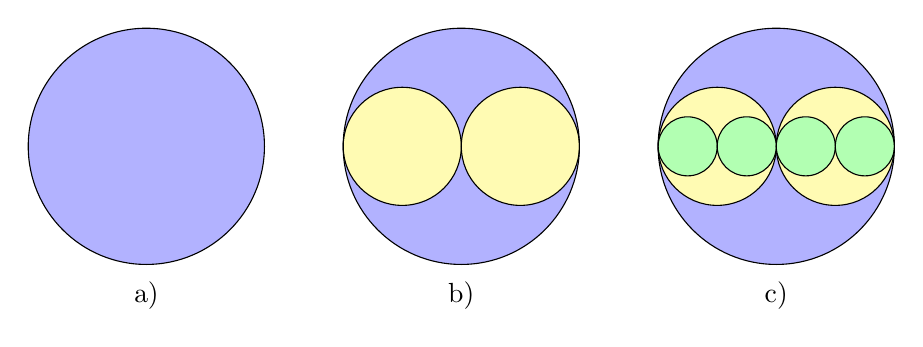
\begin{tikzpicture}
\begin{scope}
\fill[blue!30] (0,0) circle(1.5);
\draw (0,0) circle(1.5);
\node at (0,-1.9) {a)};
\end{scope}
\begin{scope}[xshift=4cm]
\fill[blue!30] (0,0) circle(1.5);
\foreach \x in {-0.75, 0.75} {
\fill[yellow!30] (\x,0) circle(0.75);
\draw (\x,0) circle(0.75);
}
\draw (0,0) circle(1.5);
\node at (0,-1.9) {b)};
\end{scope}
\begin{scope}[xshift=8cm]
\fill[blue!30] (0,0) circle(1.5);
\foreach \x in {-0.75, 0.75} {
\fill[yellow!30] (\x,0) circle(0.75);
\draw (\x,0) circle(0.75);
}
\foreach \x in {-1.125, -0.375, 0.375, 1.125} {
\fill[green!30] (\x,0) circle(0.375);
\draw (\x,0) circle(0.375);
}
\draw (0,0) circle(1.5);
\node at (0,-1.9) {c)};
\end{scope}
\end{tikzpicture}
\end{center}

% \shortans{$628$}
\loigiai{
Gọi $u_1$ là diện tích của hình tròn đầu tiên, ta có $u_1 = \pi R^2$.	\\
Gọi $u_2$ là tổng diện tích của $2$ hình tròn cắt lần thứ hai, ta có $u_2 = 2 \pi \left( \dfrac{R}{2} \right)^2 = \pi R^2 \cdot \dfrac{1}{2}$.	\\
Gọi $u_3$ là tổng diện tích của $4$ hình tròn cắt lần thứ ba, ta có $u_3 = 4 \pi \left( \dfrac{R}{4} \right)^2 = \pi R^2 \cdot \dfrac{1}{4}$.	\\
...
Gọi $u_n$ là tổng diện tích của $2^{n-1}$ hình tròn cắt lần thứ $n$, ta có $u_n = 2^{n-1} \pi \left( \dfrac{R}{2^{n-1}} \right)^2 = \pi R^2 \cdot \dfrac{1}{2^{n-1}}$.	\\
Dãy $u_1$, $u_2$, $\ldots$, $u_2$, $\ldots$ lập thành một cấp số nhân lùi vô hạn có $u_1=\pi R^2$ và công bội $q=dfrac{1}{2}$.\\
Vậy tổng diện tích của các hình tròn là
\[
S = \pi R^2 + \pi R^2 \cdot \dfrac{1}{2} + \pi R^2 \cdot \dfrac{1}{4} + \ldots = \dfrac{\pi R^2}{1 - \dfrac{1}{2}} = 2 \pi R^2 = 2 \pi \cdot 10^2 \approx 628.
\]
}
\end{ex}

% \indapan{3}{ans/11-CK1-THPT-Vinh-Xuan-Vinh-Long-Phan-1}







